\chapter{Behavioral and Neurophysiological Representations of Speech Phonemic Units}\label{ch:adrielledecar3}
\chapterauthor[1]{Adrielle C. Santana}
\chapterauthor[2]{Adriano V. Barbosa}
\chapterauthor[3]{Hani C. Yehia}
\chapterauthor[4]{Rafael Laboissière}
\begin{affils} 
\chapteraffil[1]{Universidade Federal de Ouro Preto}
\chapteraffil[2]{Universidade Federal de Minas Gerais}
\chapteraffil[3]{Université Grenoble Alpes}
\end{affils}

%%%%%%%%%%%%%%%%%%%%%%%%%%%%%%%%%%%%%%%%%%%%%%%%%%%%%%%%%%%%%%%%%%%%%%
\section*{Introduction}
\label{sec:intro}
Many studies showed that we perceive the world around us by categorizing the
sensory input. This was studied, for example, for the perception of emotions
\citep{mccullough2009categorical} and speech \citep{liberman1957discrimination}.

For centuries, researchers around the world try to understand how our brain
process speech and they try to propose a neurobiological model that explains
the mechanisms that underlie the production-perception relationship. The
dual-stream model is one example \citep{hickok2007cortical}. But how such
models relate or explain the categorical perception of speech? Many works tried
to address this issue.

In the works of \citet{alho2016early, chevillet2013automatic} and
\citet{mottonen2014attention} the authors worked with a continua based on
formant variations. In general, in those works the authors concluded about a
sensorimotor integration of auditory and motor areas for early categorization
which will occur around $120 - 170~ms$ after stimulus onset. In \citet{Bouton},
for a similar continuum, the authors identified the encoding of the second
formant frequency around $95-120~ms$ and again at $175~ms$. In
\citet{bidelman2013} the authors synthesized an /u/-/a/ continuum and observed
categorical perception around $175~ms$ after stimulus onset. With this same
continuum \citet{bidelman2017} concluded that the phonemic categorization was
dependent of attention. However, in \citet{chang2010categorical} the authors
identified the phonemic categorization around $110~ms$ in a task without
attention (passive).

Based on those works we propose to perform the investigation of the neural
correlates of categorical perception of speech sounds taking into account the
attention and the acoustic cue influence as well the brain region measured. We
also observed that the works reviewed selected the continuum \textit{a priori}
and did not performed any kind of dissociation of the physical ($\phi$) and
psychophysical ($\psi$) characteristics of the stimuli, so we took into account
these issues in our study as well.

In order to perform this dissociation we considered the hypothesis illustrated
in the Figure \ref{cat}. It shows four stimuli in a phonemic continuum, in this
example between the syllables $/da/$ and $/ta/$, differing in the Voice Onset
Time (VOT). The physical values of VOT is represented in the horizontal axis.
The vertical axis shows the probability of $/ta/$ responses in an
identification task. The first (blue) and last (red) stimuli would be
unambiguously identified as either $/da/$ or $/ta/$. However, the central
stimuli (yellow and green), which are close to each other in terms of physical
characteristics, would be represented rather distantly from each other in the
psychophysical domain. Then, we hypothesize that is possible to identify two
separate axes in the neurophysiological space: one related to the physical
characteristics of the stimuli and another related to its psychophysical
categorical perception. 

\begin{figure}
\centering
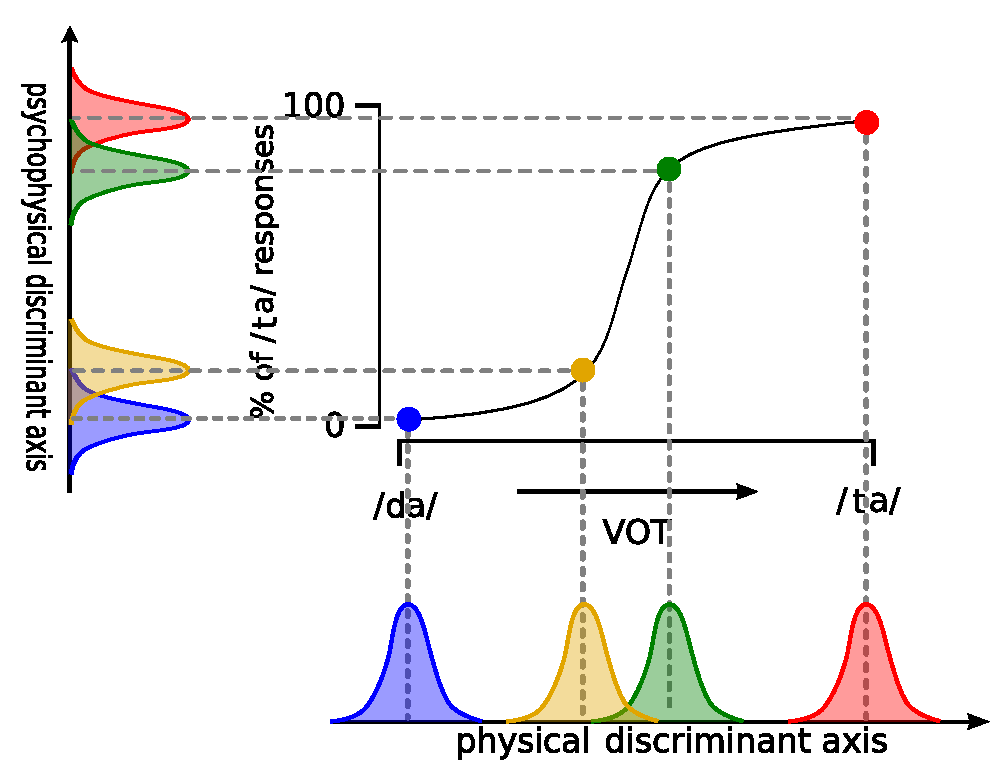
\includegraphics[width=\linewidth]{imgs/categ.pdf}
\caption{Physical and psychophysical (categorical) neurophysiological axes for
the $/da/-/ta/$ continuum. The physical values of VOT is represented in the
horizontal axis. In the vertical axis, is represented the probability of $/ta/$
responses in an identification task.} \label{cat}
\end{figure} 



%%%%%%%%%%%%%%%%%%%%%%%%%%%%%%%%%%%%%%%%%%%%%%%%%%%%%%%%%%%%%%%%%%%%%%
\section*{Methodology}
\label{sec:Methodology} 

We performed electroencephalogram (EEG) acquisitions in eleven participants,
right-handed and measured five signals from the electrodes difference: Cz--Tp9,
Cz--Tp10, Cz--Fz, Cz--F7 and Cz--F8. The experiments were randomized across
participants and each one performed both tasks (passive or active) with both
continua (based on VOT variations or formants variations). For the acquisitions
we selected five stimuli based on the psychometric curve of each subject for
each continuum as represented in Figure \ref{psy} or a given participant.

\begin{figure}
\centering
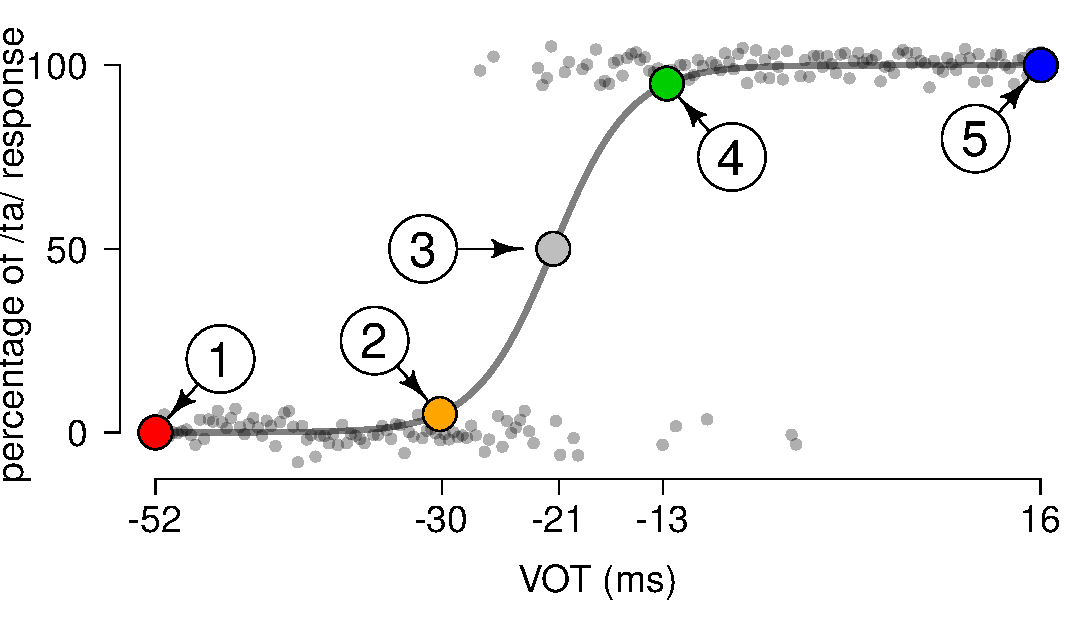
\includegraphics[width=\linewidth]{imgs/VOT-S04.pdf}
\caption{Psychometric curve for a given subject, for the VOT-continuum and the
five stimuli selected} \label{psy}
\end{figure}


%%%%%%%%%%%%%%%%%%%%%%%%%%%%%%%%%%%%%%%%%%%%%%%%%%%%%%%%%%%%%%%%%%%%%%
\subsection*{Time-domain processing}

To evaluate how the brain oscillations are involved in the coding of the
acoustic cues e to obtain the $\phi$ and $\psi$ representations of the stimuli
is interesting to work in the time-frequency domain.

For the processing we organized the data by electrode, participant, stimuli,
continuum and task. The data was resampled for the execution of the Discrete
Wavelet Transform (DWT) with decomposition in 9 levels. This way, the last
levels presented a bands similar to those of the main brain oscillations
($\delta, \theta, \alpha, \beta$ and $\gamma$).

In general, we want to relate the behavior (observed in the psychometric curve)
with the neural representation for each participant. However we arrived in a
High Dimension Low Sample Size (HDLSS) problem with five observations and $800$
wavelet coefficients (features). Then, we developed a regression technique to
address this problem named Regression on Low-Dimension Spanned Input Space
(RoLDSIS) \citep{santana2020bmc}. Then we were able to obtain the $\phi$ and
$\psi$ neural discriminant axes which we evaluated in two ways: through the
angle between them and through the Euclidean distance between them, which we
called \emph{discrepancy}.


With the angle we compared how it relate with the slope of the psychometric
curve, which is reported as a measure of the categorical perception of the
participant \citep{bidelman2017}. With the discrepancy analysis we worked with
its value in different regions of the scalogram (graphical representation of
the DWT), related to the N1 and P2 latencies and the main brain oscillations as
illustrated in Figure \ref{ROIs}. We obtained mixed-effects models for each
region considering factors related to the continuum, task and electrodes, then
we performed an ANOVA followed by a contrast analysis of the factors which
presented significant effects.

\begin{figure}
\centering
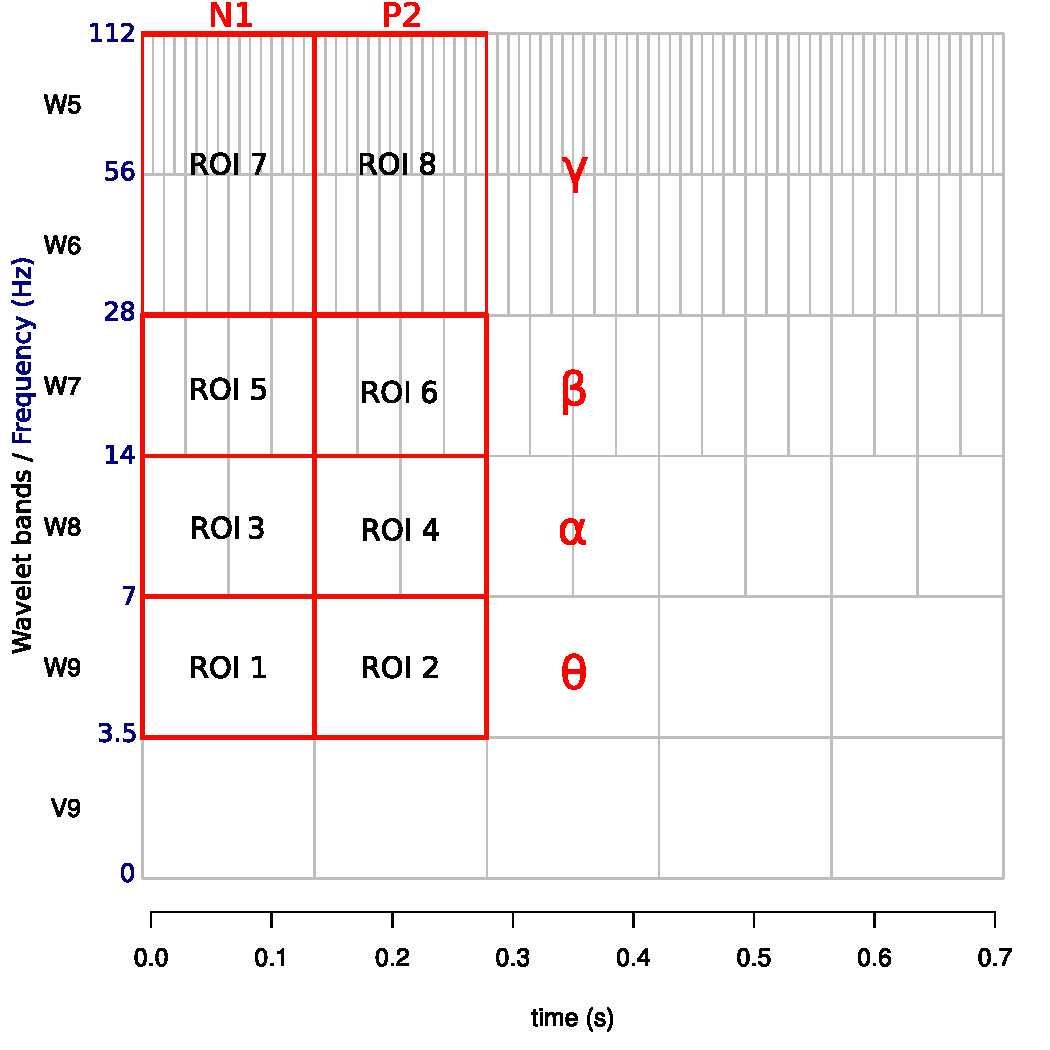
\includegraphics[width=\linewidth]{imgs/ROIs.pdf}
\caption{Definition of the ROIs as dependent variables for the models. Each ROI
corresponds to specific a frequency band and specific a time interval.}
\label{ROIs}
\end{figure}




%%%%%%%%%%%%%%%%%%%%%%%%%%%%%%%%%%%%%%%%%%%%%%%%%%%%%%%%%%%%%%%%%%%%%%
\section*{Results}
\label{sec:resul}

\subsection*{Time-domain results}
Following it will be reported our main results for our time-domain analysis and
some works that corroborate what we observed.

\begin{itemize*}
\item We observed that there is a left hemisphere dominance for speech
 processing \citep{hickok2007cortical, boemio2005hierarchical}; \item A
 spectrotemporal analysis of the acoustic cue happens at the temporal region
 \citep{hickok2007cortical};
\item Generators of N1 and P2 are more laterally localized; \item Formants and
 VOT evoke different behaviors in N1 and P2 generators;
\item N1 is sensitive to VOT variations \citep{steinschneider1995physiologic,
 eggermont1995representation}; \item Stimuli are processed differently when
 there is attention to the task and attention influences the speed of
 stimuli processing
\citep{mottonen2014attention, alho2016early};
\item Ambiguity is reflected into ERP amplitudes \citep{bidelman2017} \item P2
 seems to code ambiguity or effort for speech perception
 \citep{rao2010selective};
\item Attention influences the generators recruited to process stimuli
 \citep{hillyard1973electrical}; \item Attention influences more left
 hemisphere generators than right ones.
\end{itemize*}

\subsection*{Time-frequency domain results}
Following it will be reported our main results for our time-frequency domain
analysis.

\begin{itemize*} 
\item Participants which categorize better have larger
 difference in internal $\phi$ and $\psi$ neural representations of acoustic
 cues. The Figure \ref{formAct} illustrates the positive and significant
 correlation (r=0.788) between the axes' angles and the slopes of the
 psychometric curve for the formant continuum with the active task; \item It
 was observed a more lateral location of the speech structures;
\item $\gamma$ activity was observed in all scalp regions measured and this is
 probably related to integration/synchronization of these regions; \item
 Enhancement of $\alpha$ activity with attention; \item Larger discrepancies
 associated with the temporal region than the frontal or medial one; \item
 Brain oscillations involved in high level speech processing present strong
 activity as early as the N1 time frame.
\end{itemize*}

\begin{figure}
\centering
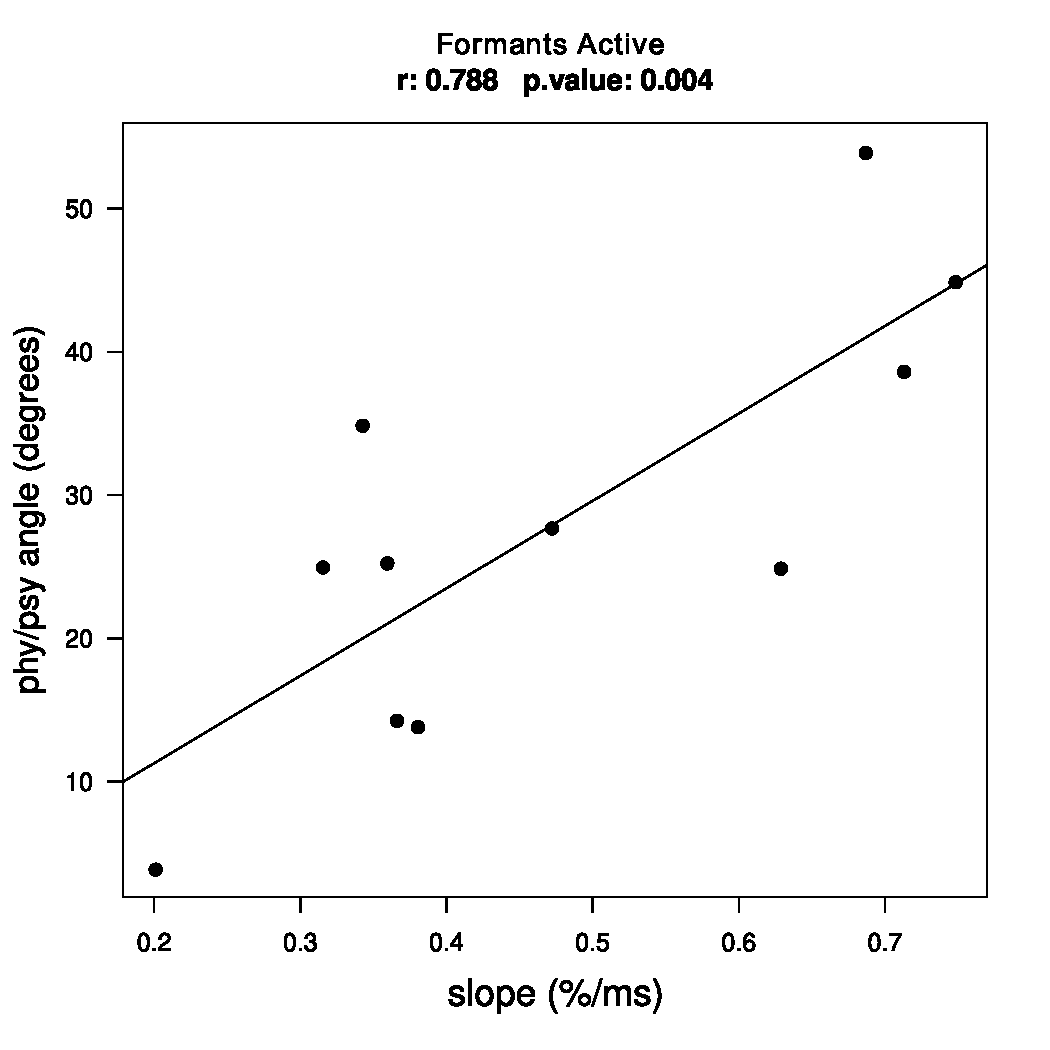
\includegraphics[width=\linewidth]{imgs/Formantes-Ativo-slope-angle.pdf}
\caption{Relationship between the slope of the psychometric
curve and the angle between the neurophysiological axes. In this
population scatter plot, each point represents a participant. The
horizontal and vertical axes represent, respectively, the slope of
the fitted psychometric curve at 50\% and the angle between the
physical and the psychophysical directions obtained by the RoLDSIS
procedure. The black line corresponds to the correlation line.}
\label{formAct}
\end{figure}


%%%%%%%%%%%%%%%%%%%%%%%%%%%%%%%%%%%%%%%%%%%%%%%%%%%%%%%%%%%%%%%%%%%%%%

\section*{Conclusions}
\label{sec:concl}
In this work we investigated the neural correlates of categorical perception of
speech sounds, specifically of Brazilian Portuguese phonemes, evaluating ERPs
in the scope of the stimulus acoustic characteristic (VOT and formant
frequencies). We studied the brain cortical regions involved in speech
perception (temporal and frontal), manipulating the degree of attention to the
identification task and using data acquired with the use of a non-invasive
method. In our analysis, we propose to identify the physical and psychophysical
responses in the ERP, in order to show how the modulations in the time and
frequency characteristics of the ERP can be related to the phonemic categorical
perception (CP).

We saw that each frequency band and latency seems to code different aspects of
the sound for the speech processing. It was observed that participants who
presented behaviorally stronger CP had a larger difference between their
physical and psychophysical neural representation of the stimuli. This
difference was pronounced for the VOT acoustic cue than for the formants and
for active tasks than for the passive ones. It was also shown that the CP
occurs when there is no attention to the auditory task but only for the
formant-based acoustic cue. Hemispheric differences were observed, with
stronger activity at the left hemisphere. Differences were also observed
between frontal and temporal cortical regions coded by low-frequency rhythms
with more activity at the temporal region. In the gamma band we observed no
significant difference between the activity at the frontal and temporal
regions.

Our results also showed that temporal region structures may also perform some
categorization besides the processing of physical acoustic characteristics of
the sounds. We also show how the acoustic cue and task dynamically reconfigure
the speech network which should be took into account by a neurobiological model
for speech perception.

This study compared different factors related to categorical speech perception
in Brazilian Portuguese using a reproducible protocol developed for the study
and the evaluation of phonemic categorical perception, and confirmed many of
the results found in the literature for other languages.

%%%%%%%%%%%%%%%%%%%%%%%%%%%%%%%%%%%%%%%%%%%%%%%%%%%%%%%%%%%%%%%%%%%%%%

\section*{Data and Materials}
The data that support the findings of this study, as well as the scripts four
reproducing the results and the thesis, are available in the following repositories:

\begin{itemize*}
 \item \url{https://github.com/Adrielle-Santana/ThesisScripts}
 \item \url{https://github.com/RoLDSIS/code}
 \item \url{http://hdl.handle.net/1843/35151}
\end{itemize*}

%%%%%%%%%%%%%%%%%%%%%%%%%%%%%%%%%%%%%%%%%%%%%%%%%%%%%%%%%%%%%%%%%%%%%%

\bibliographystyle{plainnat}
\bibliography{adrielledecar3.bib}


